% !TeX spellcheck = en_US
\documentclass[a4paper]{scrartcl}
\usepackage[left=2cm, right=2cm, top=2cm, bottom=2cm]{geometry}
\usepackage{lmodern}
\usepackage{sectsty}
\usepackage[T1]{fontenc}
\usepackage[utf8]{inputenc}
\usepackage[english]{babel}
\usepackage{tabularx}
\usepackage[dvipsnames]{xcolor}
\usepackage{dirtree}
\usepackage[hidelinks]{hyperref}
\usepackage{algpseudocode}
\usepackage{algorithm}
\usepackage{algorithmicx}
\usepackage{tikz}
\usetikzlibrary{automata, positioning, arrows, shapes.geometric}

\usepackage{xcolor}
\usepackage{scrhack}
\usepackage{listings}

\usepackage{tcolorbox}

\allsectionsfont{\sffamily}

\newcommand{\file}[1]{\texttt{#1}}
\newcommand{\program}[1]{\textbf{#1}}
\newcommand{\variable}[1]{'\texttt{#1}'}
\newcommand{\module}[1]{\texttt{#1}}
\newcommand{\script}[1]{\texttt{#1}}

\newcommand{\green}[1]{\textcolor{green}{#1}}

\newenvironment{notebox}
	{\begin{tcolorbox}\textsf{\textbf{Note:}}\\}
	{\end{tcolorbox}}

\title{Version 2 of the TSClient LEGACY Package Manager}
\subtitle{Developer's documentation}
\author{Thomas Erbesdobler <t.erbesdobler@gmx.de>}

\begin{document}
	\maketitle
	\tableofcontents
	
	
	\section{Introduction}
	\label{sec:introduction}
	
	Over the last two years (it's spring 2020) TSClient LEGACY has improved a lot. Though I cannot show you something yet. But the new build system requires a better package manager. Not that the TPM would be bad, but it's simply too slow and, most important as the time of this writing, does not allow to install packages when their files are already present. This makes it harder to bootstrap a system. I.e. one would have to install the bootstrapping toolchain into a different directory and adapt it after installing the final dynamic linker so that the compiler uses this one and lets the INTERP program header point to the correct interpreter.
	
	I think bootstrapping a system on the fly would be pretty cool, and hence I decided to rewrite the TPM in C++. I actually knew right after a few days working on and using the original TPM that I will have to do this one day, when I'll reach the limits of my Ocaml code as well as of the xml-based package database. So the primary new features that should come with this rewrite are the following (and I wanted all of them back then):
	
	\begin{itemize}
		\item A faster package database. Namely I'm going to use Sqlite3.
		\item The ability to adopt existing files. Not sure if this was the original plan back then, but I always felt like I need a better way to find conflicting packages than checking if their files are already in place before unpacking them.
		\item Source package version numbers shall be supported by the package manager. I always want it to be as slim as possible and not getting bloated with other stuff a package manager should not handle, but this seems very essential. Especially as the binary version numbers are difficult to understand in the context of microversioning. And I definitely don't want to end up doing something like \textit{"openssl-1.0.1h-2020.48.3097623"}.
		\item Truly support moving files between packages and therefore truly support conflicting packages. That is somewhat linked with adopting existing files as it requires the common base: conflicting packages.
		\item Not sure but I don't think the Ocaml code is exactly bleeding edge fast.
		\item More maintainer scripts (borrowed that term from Debian) and a more sensible way of using them (look at what rpm / dpkg does ...).
	\end{itemize}

	So, this document will contain the developer's documentation. That is especially internals and design decisions, but most important algorithms, concepts and maybe file formats, and a lot more if it comes into my vision.
	
	
	\section{depres}
	\label{sec:depres}
	
	First, I would like to talk about \module{depres}, which is the module that handles dependency resolution. The core of it is the dependency resolving algorithm, let me call it the depres-algorithm. It's input is a set of installed packages and a set of new packages that should be installed. It then constructs an installation graph from that through adding missing dependencies of the packages and choosing versions of packages to install. As second optimization goal apart from finding a feasible configuration of package versions such that all dependencies are fulfilled it tries to minimize the number of packages that need to be upgraded or installed. This distinguishes the conventional depres-algorithm from one used for upgrading all packages, which of course tries to maximize the number of upgraded packages.
	
	Before talking about the algorithm it is probably a good idea to explain my notion of dependencies.
	
	
	\subsection{Dependencies and dependency lists}
	\label{ssec:dependencies_and_dependency_lists}
	
	A dependency is a pair of the package (name and architecture) on which shall be depended and a predicate that constrains the accepted versions of that package. This is usually a predicate-logical formula made of and- and or connected less-/bigger-/equal predicates on the destination package's version. Practically I would implement this as a struct (or class; it's the same in C++ anyway) with the name as member and maybe a list of lists that represents the formula in CNF or DNF. Maybe I could also translate an arbitrary formula to objects representing and- and or operators by objects that have two children and so on. The former is probably easier (actually faster) to verify against a given version number because not the entire syntax tree of the formula needs to be parsed. But the latter could be easier to maintain, given that usually during parsing the packed form of a package constraints are only added and not deleted. One thing is however clear: the latter cannot be represented by vectors. Anyway, I'll see.
	
	Such a dependency describes one package to depend on. Now a dependency list is simply a list of such dependencies with each describing a different package. I don't think it must be anything special as no lookups will probably be done in that list. As there are binary- and source version dependencies, a package's dependencies can be described by two lists.
	
	Having said that I can now talk about the depres-algorithm.
	
	
	\subsection{The depres-algorithm}
	\label{ssec:the_depres_algorithm}
	
	It's probably similar to the original depres-algorithm used in the original TPM's depres \module{depres} module.
	
	The algorithm maintains an installation graph and a set of 'active' packages. A package is 'active' if it's version is not decided upon yet and/or its dependencies were not added to the graph yet. This can also mean that a version has been chosen but the algorithm did not yet verify if it still fulfills the requirements. The installation graph's nodes represent packages in two different states: installed already or to be installed / upgraded. Additionally if the algorithm installs a package, it stores why it decided to do so to distinguish between automatically- and manually installed packages. Each node is annotated with the currently chosen package version and predicate that specifies the accepted versions of that package. It's similar to the one used for dependencies, but each sub-predicate needs to be annotated with the package that imposed it. Therefore using a conjunction of multiple clauses is better here because each clause can then be attributed to a package. It is important to store that information as the requirements of packages may change as they are upgraded. That means removing old dependencies and adding new ones.
	
	Installing and upgrading packages can introduce conflicting packages into the system. I think the package manager should be able to deal with them as long as older or automatically installed packages will or can be removed during installation. This begs the question when these packages should be removed. I would say just before the conflicting packages will be installed to keep them as long as possible. This requires unconfiguring them and removing files that will not be overwritten by the new package. Other files should be kept to allow a smooth transition. However I'm pretty sure that this is not enough and removing manually installed packages needs to be allowed, too. Consider i.e. packages A and B that do not conflict. Now there is a new package C that replaces both. A and B may be manually installed ...
	
	Initially the installation graph is empty. The algorithm adds all installed packages and their version numbers. It adds all dependencies of the installed packages as edges and to the packages' formulas. After that the installation graph represents the current situation. I can do a check if the configuration is valid by verifying that the chosen versions fulfill the formulas and they do not conflict, and abort early if that's not the case, leaving the residing work to a repair operation.
	
	Then all requested packages are added to the graph as nodes, but not their dependencies. And the algorithm adds them to the set of active packages. Now while the set is not empty, remove a package from it and locate it in the graph. If no specific version is chosen yet or if the chosen version does not fulfill the formula, add all its dependencies by introducing new edges to existing packages or finding and adding new packages to the graph that are not installed yet. The latter's dependencies don't need to be considered yet. The current package's however are added to the constraint lists as well. And every dependency is added to the set of active packages as it's version constraining formula might have changed. After all the resulting installation graph represents a feasible situation because every dependency and every constraint that goes with them was added to the graph and every package was checked against these constraints at least once.
	
	The algorithm's running time is at least $\mathcal{O}(n)$ with number of packages as $n$ since all considered packages need to be added to the graph. Moreover the algorithm performs multiple rounds until the set of installed packages is empty. I prefer a deterministic set datastructure here, hence every set-operation will be $\mathcal{O}(\log{}n)$. In each round a package is removed and all its dependencies are added if and only if the package did not fulfill the imposed version formula. This leads to an exponential running time. In practice however I think it will be rarely the case that multiple versions need to be tried. If the first version suffices for each package, each package will never be added to the set again after having been removed \textbf{and} after all packages are in the graph. So when a package is added the set may grow to size $\mathcal{O}(n)$ again. This can happen $\mathcal{O}(n)$ times leading to a practical running time of $\mathcal{O}(n^2)$, but with super-exponential worst case if all versions need to be tried and the number of versions is linear in the number of packages (could happen as both may be linear in lifetime).
	
	\paragraph{Removing conflicting packages} Whenever a (not already installed) package is added to the installation graph it may conflict with another one. I have to check that with every package (does not increase already quadratic running time) and remove the ones that conflict with the package as well as their dependency-edges and their constraint predicates in the version constraining formulas. A message to the user that can optionally be ignored would be nice. Add all reverse dependencies to the set of active packages. Then, whenever a package is removed from that set and processed in a round, it could bring the old package back (unless there is an 'or'-dependency). The algorithm can try a different version, especially as newer versions may have updated dependencies that reflect the newer package base that in turn created that conflict with packages from an older base, but if that fails it must abort when it recognizes that the situation cannot be solved as long as a certain new package needs to be installed.
	
	So different versions of all packages that depend on a removed one potentially need to be tried again and therefore all these packages need to be added to the set. This can be done by starting a DFS at the removed package that traverses edges in reverse direction. To make this work the algorithm needs to try different versions first before declaring a conflict.
	
	
	\vspace{1eM}
	Before I try further things I want to make the algorithm more concrete.
	
	\begin{algorithm}[ht]
		\caption{Pseudo code of the depres-algorithm}
		\label{alg:pseudo_code_of_the_depres_algorithm}
		
		\begin{algorithmic}
			\State $active\gets \emptyset$
			\State $V\gets \emptyset$
			\State $E\gets \emptyset$
			\State $G\gets (V, E)$
			
			\For{$p\in installed\_packages$}
				\State $V\gets V\cup \{p\}$
			\EndFor
				
			\For{$p\in installed\_packages$}
				\For{$d\in p.dependencies$}
					\State $E\gets E\cup \{(p,d)\}$
				\EndFor
			\EndFor
			\State $\vdots$
		\end{algorithmic}
	\end{algorithm}


	\subsection{Pre-dependencies vs. dependencies}
	\label{sec:pre_dependencies_vs_dependencies}
	
	There are two flavors of dependencies between packages. The more usual dependencies declare required packages at configure stage, while the dependencies need not be fulfilled during the preinst script and extracting. That means packages can be extracted and their preinst script be run in any order and the package manager ensures that dependencies are met only for configuration and later installed packages. A preinst script however could require other packages, too. It usually will at least need an interpreter, therefore requiring a dependency facility before a package's installation begins. The TPM2 achieves this (like Debian's dpkg and rpm) through pre-dependencies. They are handles in the same way like regular dependencies but ensured before the preinst script is run. Of course cycles here must be broken at a point and hence cannot be fulfilled.
	
	There is one more important case that I would like to note here: pre-dependencies could require the same package as regular dependencies. But the required version must be the same, otherwise the package manager would have to change a dependency's version during the installation of the dependent package. I can't think of a legitimate use case for this, and avoiding that makes things easier. The installation graph needs only one set of nodes.
	
	Additionally pre-dependencies should also be available to the postrm script as the package is not configured anymore when the package manager runs it. Hence it is probably a good idea to keep them while the depending package is installed to avoid having to install another package first before a package can be uninstalled.
	
	
	\section{PackageDB}
	\label{sec:packagedb}
	
	''\module{PackageDB}'' or ''\module{package\_db}'' is the package manager's database, which stores the installed packages, their states and which files are installed. The latter is especially interesting since one has to decide which attributes of files to store. Currently PackageDB uses SQLite3 as DBMS and the following SQL relational schema (version 1.2):
	
	\begin{table}[H]
		\centering
		
		{
		\setlength{\extrarowheight}{0.5eM}
		\sffamily
		\hyphenchar\font=-1
		\begin{tabularx}{\textwidth}{lX}
			schema\_version: & \underline{version:varchar} \\
			packages: & \underline{name:varchar}, \underline{architecture:integer}, \underline{version:varchar}, source\_version:varchar, installation\_reason:integer, state:integer \\
			
			files: & \underline{path:varchar}, \underline{pkg\_name:varchar}, \underline{pkg\_architecture:integer}, \underline{version:varchar}, type:integer, digest:varchar \\
			
			config\_files: & \underline{path:varchar}, \underline{pkg\_name:varchar}, \underline{pkg\_architecture:integer}, \underline{version:varchar} \\
			
			pre\_dependencies: & \underline{pkg\_name:varchar}, \underline{pkg\_architecture:integer}, \underline{pkg\_version:varchar}, \underline{name:varchar}, \underline{architecture:integer}, constraints:varchar \\
			dependencies: & \underline{pkg\_name:varchar}, \underline{pkg\_architecture:integer}, \underline{pkg\_version:varchar}, \underline{name:varchar}, \underline{architecture:integer}, constraints:varchar \\
			
			triggers\_activate & \underline{pkg\_name:varchar}, \underline{pkg\_architecture:integer}, \underline{version:varchar}, \underline{trigger:varchar} \\
			triggers\_interest & \underline{pkg\_name:varchar}, \underline{pkg\_architecture:integer}, \underline{version:varchar}, \underline{trigger:varchar} \\
			
			triggers\_activated & \underline{trigger:varchar} \\
		\end{tabularx}
		}
	
		\vspace{0.5eM}
		\begin{flushleft}
			\textsf{triggers\_interest} has a non-unique index on \textsf{trigger}.
		\end{flushleft}
	
		\vspace{1eM}
		The type of files maybe one out of:
		
		\vspace{0.5eM}
		\begin{tabular}{c|l}
			Type & Description \\
			\hline
			0x00 & Regular file \\
			0x01 & Directory \\
			0x02 & Symbolic link \\
			0x03 & Character device \\
			0x04 & Block device \\
			0x05 & Socket \\
			0x06 & Pipe \\
		\end{tabular}
	
		\caption{Version 1.2 of \module{PackageDB}'s database schema}
		\label{tab:the_database_schema_of_packagedb}
	\end{table}
	
	It does not store file attributes at all. This deviates from the aforementioned ideal of a package manager which knows all files, but makes the implementation easier. At least for now I don't see why having the stricter version could bring a big benefit in my current and mid-term practice. If that arises it can easily be added due to versioned db schemata, anyway. The digest field contains a hash of the file's content. It may (at some point in the future when I or someone else implements this) be prefixed with something like ''\texttt{sha512:}'' to indicate the used algorithm. If no prefix is present, the algorithm shall be sha1. It's not like super-safety but a considerable measure of integrity protection.
	
	Note that all attributes of 'config\_files' could be a foreign key referencing 'files'. However later one may add support for config files which are not included in the package's archive (e.g. created by maintainer scripts) and 
	
	
	\subsection{Storing constraints}
	\label{ssec:storing_constraints}
	
	Constraints are predicate logical formulae. To easily store them, they can be converted to an invertible string representation. This allows for very compact storage compared to storing i.e. every predicate in a separate tuple. An only drawback may be that db-level analysis cannot be performed on them, but I see no interesting use case for this now. At least none that must be that fast that reading the entire table and processing it in memory cannot be justified with complexity reduction. Those applications may read the constraints together with the rest of the packages, anyway, and then it's just a question of which representation is faster, and again, there are not that many packages ...
	
	
	\subsection{Installation reasons}
	\label{ssec:installation_reasons}
	
	Basically there are two reasons why a user wants a package to be installed:
	
	\begin{description}
		\item[auto] The package was installed because other packages depend on it.
		\item[manual] The package was installed because the user wants it.
	\end{description}


	\section{Triggers}
	\label{sec:triggers}
	
	Triggers allow to run procedures required by many packages only once at the end of the package manager's execution. TPM2's trigger-concept is inspired by dpkg's. Note that RPM has triggers, too, but follows a different concept.
	
	In TPM2 triggers exist beneath packages. They can be activated and will be executed at the end of \program{tpm2}'s run. Triggers are always triggered by a package when it changes state, therefore Packages can declare in their metadata to activate triggers (see \ref{fig:the_format_of_desc_xml}). A specified trigger will be activated after the package has been configured, unconfigured or its files have been removed. TPM2 collects all triggers activated during a run in the database (s.t. it can be aborted and will not loose triggers) and executes them right before exiting successfully.
	
	Packages can declare interest in triggers in their metadata to have their \texttt{configure} script called when triggers are executed:
	
	\begin{lstlisting}[language=bash]
		configure triggered <trigger name>
	\end{lstlisting}
	
	\texttt{configure} will be called once at the end of the run for every activated trigger the package declares interest in, however note that a trigger may be activated after unconfiguring a package and removing its files, therefore \texttt{configure} could be called multiple times if TPM2 is interrupted. Hence the actions a triggered package performs must be idempotent.
	
	Apart from the list of activated triggers ('activated' is used as a synonym for 'triggered' here), PackageDB must also store the triggers a package is interested in and which it activates. The former must support an efficient lookup of packages interested in a particular trigger s.t. executing the trigger is cheap.
	
	\begin{notebox}
		A package can trigger itself. If it is interested in a trigger which it activates as well, it will be triggered at the end of \program{tpm2}'s run.
	\end{notebox}
	
	
	\section{Package states}
	\label{sec:package_states}
	
	At any point in time a package that is part of the system has a state. This state describes if it is fully part of the system or in a, say, transitional state, where the package manager needs to do more work until the package's invariants are fulfilled. State transitions are atomic operations of the package manager. As such, these must be idempotent to allow for repeating them if they were interrupted. Figures \ref{fig:package_states_install}, \ref{fig:package_states_remove} and \ref{fig:package_states_change} describe the possible state transitions and which actions go with them when installing, removing or changing a package. The latter needs to consider the old and the new version of a package. ''change'' refers to upgrading or downgrading. As a package's files may be replaced by multiple packages or multiple packages' files may be consumed by one package, this is the most complicated procedure and it involves more than one package.
	
	In other words, as long as no conflicting packages are part of the system it's easy. Conflicting packages can be there in transient states, however not in an accepted state (i.e. configured).
	
	For Installation I would like to consider the install direction (green arrows) only for now. If one stage fails, the installation shall abort and leave the system in an unclean state to be cleaned by \texttt{--recover}. If the target system is not native, the packages shall not be configured and hence left in state configure\_begin.
	
	\begin{figure}[ht]
		\centering
		
		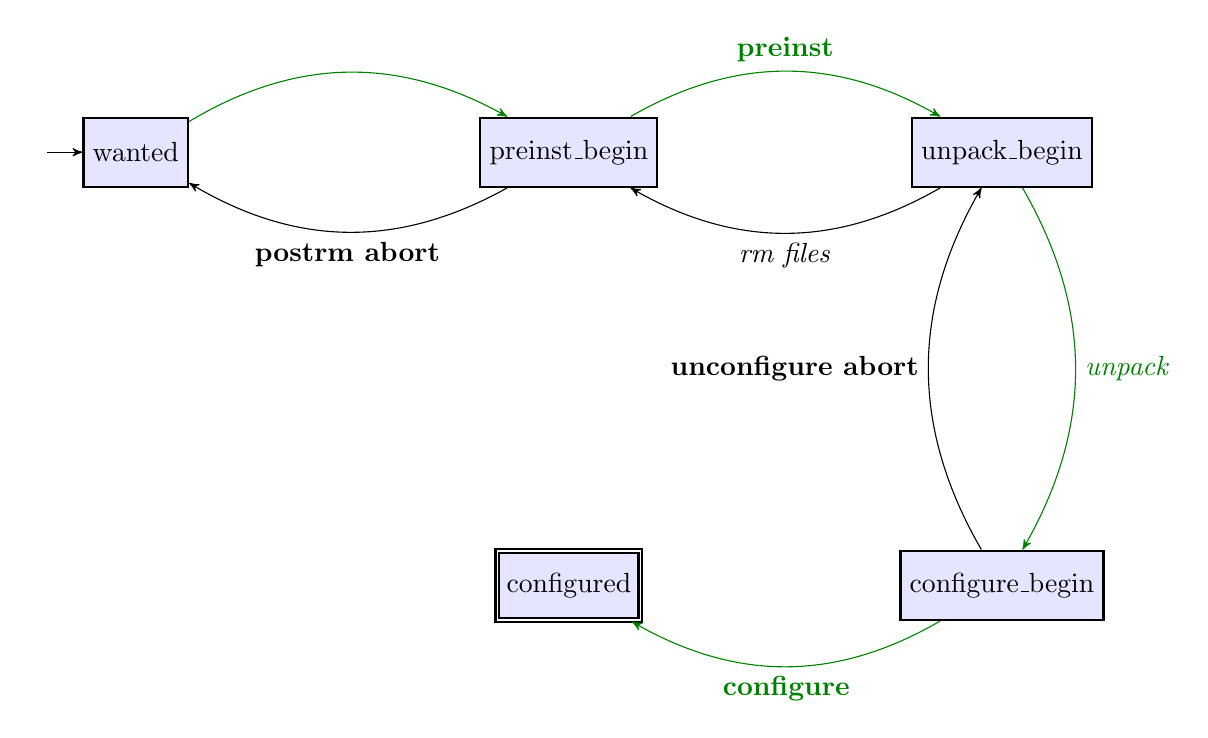
\begin{tikzpicture}[
				->,
				>=stealth',
				node distance=5.5cm,
				every state/.style={thick, fill=blue!10, rectangle},
				initial text=$ $]
			
			\node[state, initial] (wanted) {wanted};
			\node[state, right of=wanted] (preinst_begin) {preinst\_begin};
			\node[state, right of=preinst_begin] (unpack_begin) {unpack\_begin};
			\node[state, below of=unpack_begin] (configure_begin) {configure\_begin};
			\node[state, accepting, left of=configure_begin] (configured) {configured};
			
			\draw	(wanted) edge[above, bend left, color=Green] node{$ $} (preinst_begin)
					(preinst_begin) edge[below, bend left] node{\program{postrm abort}} (wanted);
					
					
			\draw	(preinst_begin) edge[above, bend left, color=Green] node{\program{preinst}} (unpack_begin)
					(unpack_begin) edge[below, bend left] node{\textit{rm files}} (preinst_begin);
					
			\draw	(unpack_begin) edge[right, bend left, color=Green] node{\textit{unpack}} (configure_begin)
					(configure_begin) edge[left, bend left] node{\program{unconfigure abort}} (unpack_begin);
					
			\draw	(configure_begin) edge[below, bend left, color=Green] node{\program{configure}} (configured);
					
			
			
		\end{tikzpicture}
		
		\caption{Package states during installation}
		\label{fig:package_states_install}
	\end{figure}

	\begin{figure}[ht]
		\centering
		
		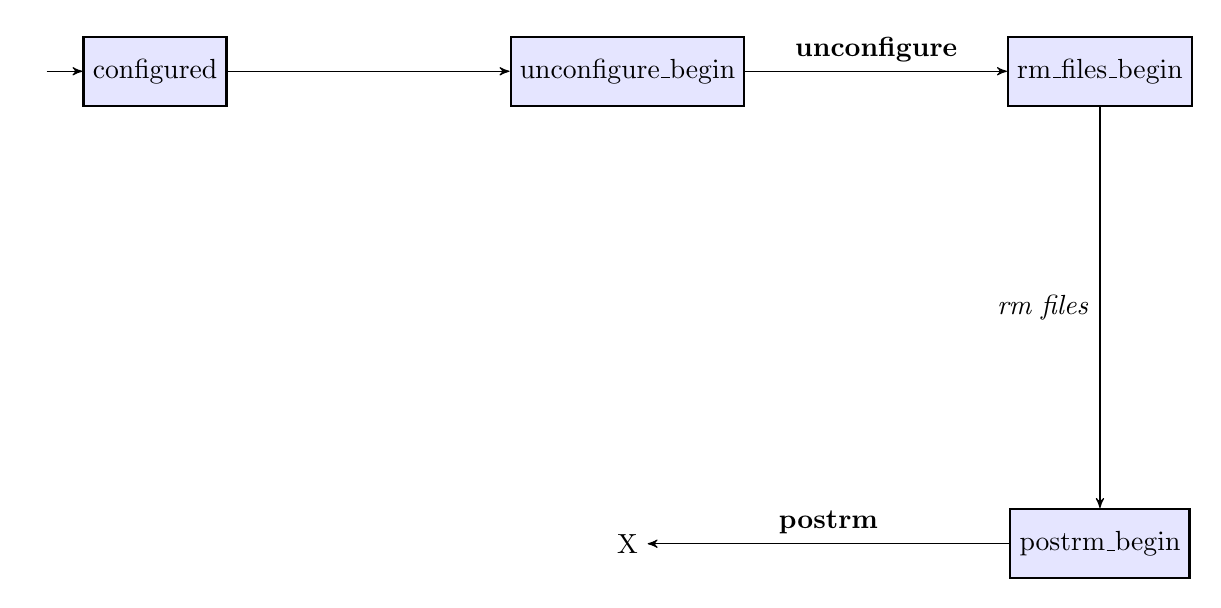
\begin{tikzpicture}[
				->,
				>=stealth',
				node distance=6cm,
				every state/.style={thick, fill=blue!10, rectangle},
				initial text=$ $]
				
			\node[state, initial] (configured) {configured};
			\node[state, right of=configured] (unconfigure_begin) {unconfigure\_begin};
			\node[state, right of=unconfigure_begin] (rm_files_begin) {rm\_files\_begin};
			\node[state, below of=rm_files_begin] (postrm_begin) {postrm\_begin};
			\node[left of=postrm_begin] (X) {X};
			
			\draw	(configured) edge[above] node{$ $} (unconfigure_begin);
			
			\draw	(unconfigure_begin) edge[above] node{\program{unconfigure}} (rm_files_begin);
			
			\draw	(rm_files_begin) edge[left] node{\textit{rm files}} (postrm_begin);
			
			\draw	(postrm_begin) edge[above] node{\program{postrm}} (X);
		\end{tikzpicture}
		
		\caption{Package states during removal}
		\label{fig:package_states_remove}
	\end{figure}

	\begin{figure}[ht]
		\centering
		
		\textit{State change of the old package to be changed or replaced:}
		\vspace{1eM}
		
		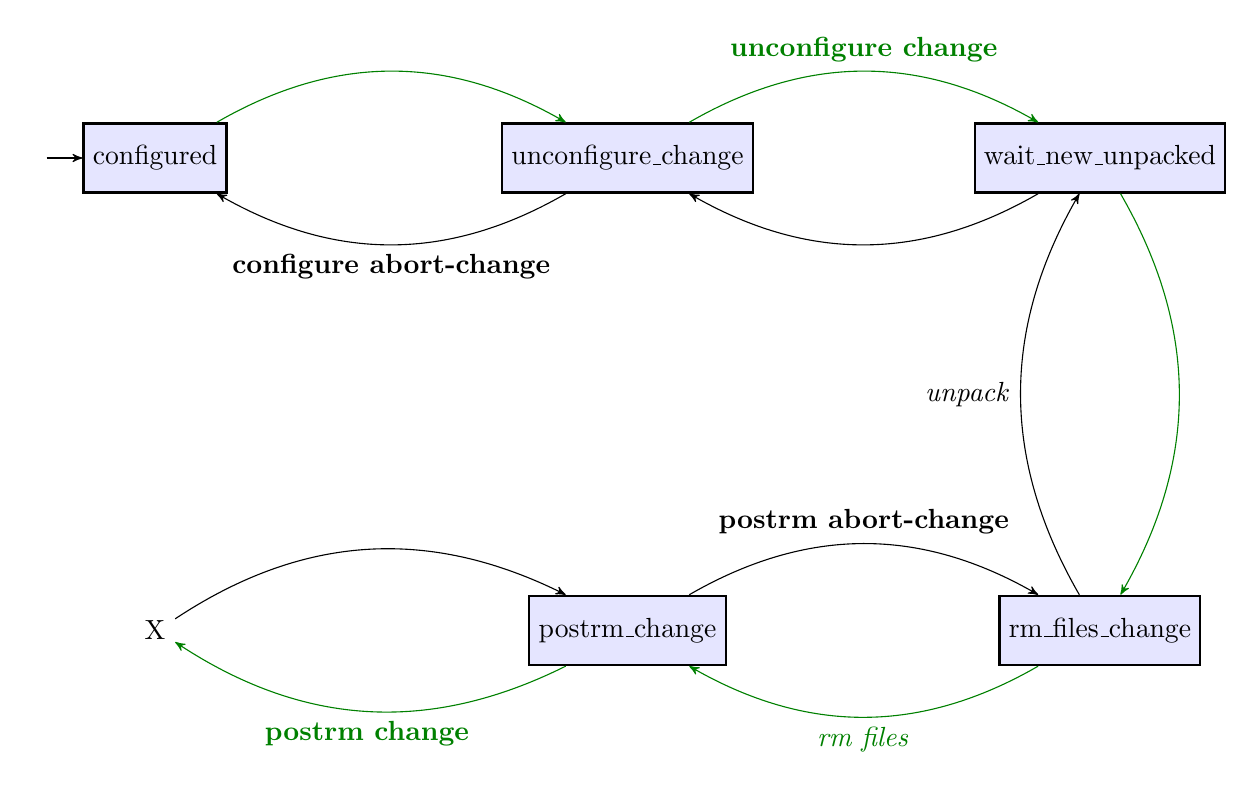
\begin{tikzpicture}[
				->,
				>=stealth',
				node distance=6cm,
				every state/.style={thick, fill=blue!10, rectangle},
				initial text=$ $]
				
			\node[state, initial] (configured) {configured};
			\node[state, right of=configured] (unconfigure_change) {unconfigure\_change};
			\node[state, right of=unconfigure_change] (wait_new_unpacked) {wait\_new\_unpacked};
			\node[state, below of=wait_new_unpacked] (rm_files_change) {rm\_files\_change};
			\node[state, left of=rm_files_change] (postrm_change) {postrm\_change};
			\node[left of=postrm_change] (X) {X};
			
			\draw	(configured) edge[above, bend left, color=Green] node{$ $} (unconfigure_change)
					(unconfigure_change) edge[below, bend left] node{\program{configure abort-change}} (configured);
					
			\draw	(unconfigure_change) edge[above, bend left, color=Green] node{\program{unconfigure change}} (wait_new_unpacked)
					(wait_new_unpacked) edge[below, bend left] node{$ $} (unconfigure_change);
					
			\draw	(wait_new_unpacked) edge[right, bend left, color=Green] node{$ $} (rm_files_change)
					(rm_files_change) edge[left, bend left] node{\textit{unpack}} (wait_new_unpacked);
					
			\draw	(rm_files_change) edge[below, bend left, color=Green] node{\textit{rm files}} (postrm_change)
					(postrm_change) edge[above, bend left] node{\program{postrm abort-change}} (rm_files_change);
					
			\draw	(postrm_change) edge[below, bend left, color=Green] node{\program{postrm change}} (X)
					(X) edge[above, bend left] node{$ $} (postrm_change);
				
		\end{tikzpicture}
		
		\vspace{1eM}
		\textit{State change of the new package:}
		\vspace{1eM}
		
		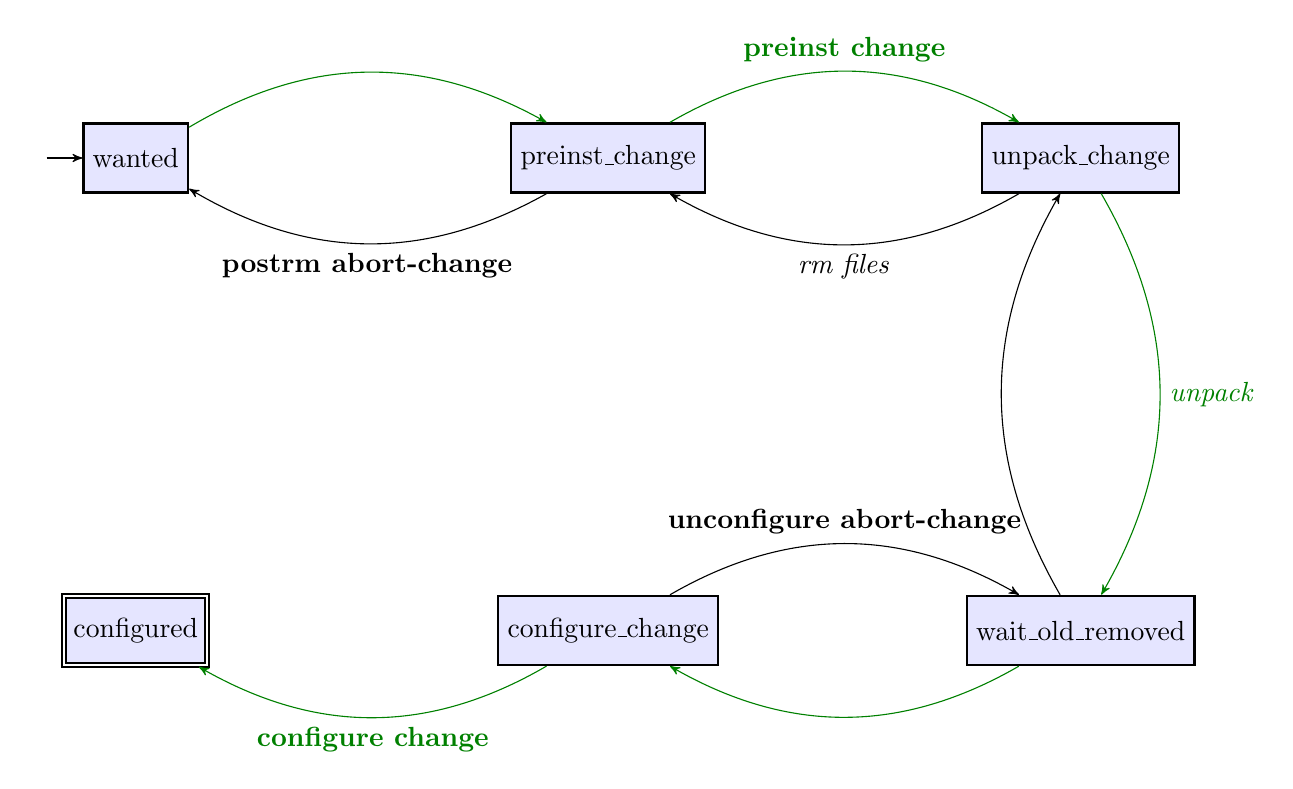
\begin{tikzpicture}[
				->,
				>=stealth',
				node distance=6cm,
				every state/.style={thick, fill=blue!10, rectangle},
				initial text=$ $]
				
			\node[state, initial] (wanted) {wanted};
			\node[state, right of=wanted] (preinst_change) {preinst\_change};
			\node[state, right of=preinst_change] (unpack_change) {unpack\_change};
			\node[state, below of=unpack_change] (wait_old_removed) {wait\_old\_removed};
			\node[state, left of=wait_old_removed] (configure_change) {configure\_change};
			\node[state, accepting, left of=configure_change] (configured) {configured};
	
			\draw	(wanted) edge[above, bend left, color=Green] node{$ $} (preinst_change)
					(preinst_change) edge[below, bend left] node{\program{postrm abort-change}} (wanted);
			
			
			\draw	(preinst_change) edge[above, bend left, color=Green] node{\program{preinst change}} (unpack_change)
					(unpack_change) edge[below, bend left] node{\textit{rm files}} (preinst_change);
			
			\draw	(unpack_change) edge[right, bend left, color=Green] node{\textit{unpack}} (wait_old_removed)
					(wait_old_removed) edge[left, bend left] node{$ $} (unpack_change);
					
			\draw	(wait_old_removed) edge[below, bend left, color=Green] node{$ $} (configure_change)
					(configure_change) edge[above, bend left] node{\program{unconfigure abort-change}} (wait_old_removed);
			
			\draw	(configure_change) edge[below, bend left, color=Green] node{\program{configure change}} (configured);
				
		\end{tikzpicture}
		
		\caption{Package states during change / replacement}
		\label{fig:package_states_change}
	\end{figure}

	The ''begin'' states are required to be undo operations only once they were started. Otherwise the package manager would i.e. have to run \program{unconfigure} again when in state unpacked, even though some files may have been removed already. \program{unconfigure} may fail then. It is not required for all states but then some operations have to redo work. That is not a problem since maintainer scripts must be idempotent anyway (consider the package manager was interrupted just before it committed to the db that a script was run). One can view the system not as having states as points in time where one operation ended and the next one will begin but one operation ended some time ago and the next one may have begun already. That indicates the direction that the last operation that induced a state change took and allows to restart from there after an interruption, only redoing this one operation rather than having to consider all directions. This limits idempotence to one operation and not one operation and its predecessor.
	
	I would not need that indication of direction if I only considered one process, like only install. But I always need at least both.
	
	The state ''wanted'' only exists because packages may lie around in memory while they're not installed yet and need to have a state. And because I did not want a tristate-like type for it. It does not need to be stored in the db.
	
	Table \ref{tab:required_package_states} summarizes the states a package can be in.
	
	\begin{table}[ht]
		\centering
		
		\begin{itemize}
			\item wanted
			\item preinst\_begin
			\item unpack\_begin
			\item configure\_begin
			\item configured
			\item unconfigure\_begin
			\item rm\_files\_begin
			\item postrm\_begin
			\item unconfigure\_change
			\item wait\_new\_unpacked
			\item rm\_files\_change
			\item postrm\_change
			\item preinst\_change
			\item unpack\_change
			\item wait\_old\_removed
			\item configure\_upgrade
		\end{itemize}
		
		\caption{Required package states}
		\label{tab:required_package_states}
	\end{table}


	\section{Files and their formats}
	\label{sec:files_and_their_formats}
	
	
	\subsection{\file{status.db}}
	\label{ssec:status.db}
	
	This is the package manager's main database in which it stores the state of the system. It is located in the \file{/var/lib/tpm} directory.


	\subsection{\file{config.xml}}
	\label{ssec:config.xml}
	
	This file configures how the package manager operates. It is located in the \file{/etc/tpm} directory.
	
	\noindent
	\dirtree{.1 <tpm file\_version=''2.0''>.
		.2 <repo type= \{dir|dir\_allow\_unsigned\}> \DTcomment{path to Directory Repository}.
		.2 <default\_arch> \DTcomment{\{i386 | amd64\}}.
	}

	
	\section{Repository formats}
	\label{sec:repository_formats}
	
	
	\subsection{Directory Repository}
	\label{ssec:directory_repository}
	
	Directory Repositories are directory trees of the following format:
	
	\vspace{1em}	
	\noindent
	\begin{tabular}{rl}
		\file{\dots/} & \file{<arch>/<package-X1\_Y1.tpm2} \\
		& \hspace{0.5cm} $\vdots$ \\
		& \file{<arch>/<package-Xn\_Yn.tpm2} \\
	\end{tabular}

	\vspace{1em}
	Their type in \file{config.xml} is \texttt{dir}.
	
	\subsubsection{Index}
	
	Directory repositories may have one or more indexes per architecture. Each index must have a unique name within the repository and architecture. It consists of two files, a metadata list named \file{<name>.index} and a file index \file{<id>.files}, which is named with a unique id referenced in the file index. This allows to regenerate the index and swap it with the old one in an atomic operation (because \texttt{rename(2)} is atomic and only one file is renamed). The shape of this id is implementation dependent. A good choice may be a timestamp, however checking if such a file exists already/creating the new one with \texttt{O\_CREAT | O\_EXCL} is always helpful.
	
	The package list is kept in a human readable format. After a file 'identifier' (like a 'magic number') with an index version (currently "1.0") follows the file index's filename and SHA256 sum (as the package list can be signed this will authenticate the file list, too). Next follows the concatenation of all package version's metadata in xml format followed by the sha256 sum of each package, and an optional signature. The order in which the package versions are listed is not important as the package list is designed to be read during \program{tpm2}'s start and held in memory. An example is given in figure \ref{fig:dir_index_package_list}.
	
	\begin{figure}
		tpm\_repo\_index 1.0 \\
		20210728120000000.files 89f250efe1058b026a23de76feea5695ae948d9511a629511f886f22990113df \\
		<pkg> \\
			\dots \\
		</pkg> \\
		89f250efe1058b026a23de76feea5695ae948d9511a629511f886f22990113df \\
		\dots \\
		</pkg> \\
		89f250efe1058b026a23de76feea5695ae948d9511a629511f886f22990113df \\
		signature \\
		
		\caption{Example package list of directory repository's index}
		\label{fig:dir_index_package_list}
	\end{figure}
	
	
	\section{About configuration files in packages}
	\label{sec:about_configuration_files_in_pacakges}
	
	Packages may contain configuration files. Not only as default configurations or usually suitable configurations but maybe also because they are usually generated by software at runtime or by an admin. I actually don't want to support a purge operation like \program{dpkg} does. And I think these at runtime created config files should be removed by maintainer scripts. For now I only support declaring files in a package as config files, which means that all config files generated at runtime have to be removed by maintainer scripts - this is a compromise. However all config files are stored in lists (without digests; those have to be retrieved from the regular file indexes) hence it should not be too difficult to add support for runtime-generated config files (without a digest as that cannot be known in advance) later on.
	
	A config file for which the digest is known (currently all config files) will only be overwritten / deleted during unpacking an archive if it was not changed or deleted. It is considered changed if its digest or type changed. Only links and regular files can be considered config files, and replacing a link with a config file or vice versa means a change in this sense. However the TPM2 does not store if a config file was recognized as changed at some point, hence if the new version matches the one on the system, the latter won't be overwritten but for future operations considered as unchanged as if it was installed by the package.
	
	By default \program{tpm2\_pack} will add all files under \file{/etc} as config files. However a file \file{config\_file\_patterns} can be added in the unpacked form's root, which contains one ECMAScript-like regular expression (interpreted by C++ 11's \texttt{std::regex}) per line against which the entire paths of the package's files will be matched. If a file matches one of the regular expressions, it is added as a config file.
	
	
	\section{different forms of packages}
	\label{sec:differnt_forms_of_packages}
	
	Packages come in three different forms or shapes: unpacked, packed/transport form and installed. The unpacked form is a more temporary construct for creating a package, it is converted to Transport Form by \program{tpm2\_pack}. When the package manager installs a package, it unpacks the transport form to the installed form where files life on the system and metadata is stored in the database. Maintainer scripts must be stored there, too, although I'm not sure how exactly, yet (basically in db or /var/lib/tpm/<pkg\_name/).
	
	In the following I would like to describe the different forms in greater detail.
	
	
	\subsection{The unpacked form}
	\label{ssec:the_unpacked_form}
	
	It's nothing magic; just a directory with a xml-file called \file{desc.xml} to hold the package metadata in its root, the maintainer scripts if present and a directory called \file{destdir} in which the package contents are to be installed. The latter can have arbitrary permissions and represents the root of the root filesystem. The format of \file{desc.xml} is described in figure \ref{fig:the_format_of_desc_xml} and this format is common to the metadata section of the transport form. The maintainer scripts have names \file{preinst}, \file{configure}, \file{unconfigure} and \file{postinst}. Their permission does not matter, too, as the package manager will extract these (if it extracts them to disk) with executable permissions.
	
	In addition to that a file \file{config\_file\_patterns} may be present, which defines how config files are identified. It contains C++11-compatible regular expressions (similar to ECMAScript) on each line against which the file's paths are matched. The full paths are matched, i.e. \texttt{\^} and \texttt{\$} are not required. Without that file, all files under \file{/etc} are considered config files by default.
	
	\begin{figure}[ht]
		\dirtree{.1 <pkg file\_version="2.0">.
			.2 <name>.
			.2 <arch> \DTcomment{\{i386 | amd64\}}.
			.2 <version> \DTcomment{The binary version; usually the ''microversion''}.
			.2 <source\_version> \DTcomment{The source version number}.
			.2 <pre-dependencies>.
			.3 <dep>.
			.4 <name>.
			.4 <arch> \DTcomment{\{i386 | amd64\}}.
			.4 <constr type="\{eq, neq, geq, leq, gt, lt\}">version</constr>.
			.4 <sconstr> \DTcomment{source version constraint}.
			.2 <dependencies>.
			.3 $\vdots$.
			.2 <triggers>.
			.3 <activate> \DTcomment{activate this trigger; can be used zero or more times}.
			.3 <interested> \DTcomment{declare interest in this trigger; can be used zero of more times}.
		}
	
		\vspace{1eM}
	
		The first four parameters (''sections'' in XML jargon) must come first to ease reading the file. For dependencies, the \texttt{name} and \texttt{arch} sections must come first. \texttt{pre-dependencies}, \texttt{dependencies} and \texttt{triggers} are optional (default to empty) but should be generated by \program{tpm2\_pack}.
		
		\caption{The format of \file{desc.xml}}
		\label{fig:the_format_of_desc_xml}
	\end{figure}
	
	
	\subsection{A new transport form}
	\label{ssec:a_new_transport_form}
	
	TPM version 1 used tar archives composed of a control file, maintainer scripts and another (compressed) tar archive as transport or packed form of packages. For TPM 2 I want to change a few things. It should just be one tar archive for the files, or rather an archive I can easily read and possibly extract (to adopt files) by hand. This removes the requirement of having a file list be duplicated together with hash sums for config files in the meta data. With TPM 2 this becomes even more important as virtually all file attributes need to be accessed by the package manager directly and not just an external archiver to decide if and if yes how to adopt files already present prior to installing a package. And I don't think I still need to extract the outer archive or single elements from it to a temporary location before reading them. I'm grown enough to do this in memory or even better on the fly with streams or something similar.
	
	So I propose the following format: The transport form consists of different sections that are concatenated together. In the beginning is a table of contents to easily seek to specific section. It also delimits the individual sections such that no special deliminating length-header like thing is required in each one. It looks like the following:
	
	\vspace{1eM}
	
	\begin{center}
		\begin{tabular}{|l|c|c|c|}
			\hline
			Address & \multicolumn{3}{c|}{data} \\
			\hline
			0x0000 & version: u8 (= 1) & count of sections: u8 & \\
			\hline
			0x0002 & section type: u8 & start: u32 & size: u32 \\
			\hline
			0x000b & section type: u8 & start: u32 & size: u32 \\
			\hline
			\multicolumn{4}{|c|}{$\vdots$} \\
			\hline
		\end{tabular}
	\end{center}
	
	\vspace{1eM}
	
	Since multi-byte integers are stored, but files usually have a word size of one byte, one needs to decide upon a serialization scheme, so big- or little endian. Everybody always says big endian or more imposing \texttt{network byte order}. I like that, too, and use it all over the place. But here I deal with a lot of little endian systems, actually in the beginning only those. So I decided to be different in that point and use little endian. Remember, that's were the more significant bytes go upwards to the higher addresses ...
	
	The futuristic may scream now '32 bit is outdated!' - but really? You ever think there'll be a package with more than 4g in the near future?

	
	\vspace{1eM}	
	I moreover need different section types:
	
	\vspace{1em}

	\begin{tabularx}{\textwidth}{c|c|X}
		Identifier & Required & Description \\
		\hline
		0x00 & yes & meta data (like former \file{desc.xml}) \\
		0x01 & no & file index \\
		0x02 & no & config files \\
		0x20 & no & \script{preinst} script \\
		0x21 & no & \script{configure} script \\
		0x22 & no & \script{unconfigure} script \\
		0x23 & no & \script{postrm} script \\
		0x80 & no & The file archive \\
		0xf0 & no & A OpenPGP signature \\
	\end{tabularx}

	\vspace{1eM}
	
	All text like scripts shall be utf8-encoded, binary data is binary data. The sections must appear in the order they're listed in the table. For the signature it's very natural to be the last part, such that it can be appended like a detached signature. For the other sections it's not that imposed but it should be at least good manner to have the metadata first. Not sure if I'll keep this strict ordering requirement forever. Well, at least the easy-to-skip parts should come first (if they ever have to be skipped) because seeking in a compressed form of such a file is very expensive.
	
	The file index must be present if and only if the archive is present. Otherwise there are simply no files associated with the package (maybe like in Debian's virtual packages). The index's format is described in figure \ref{fig:the_file_index_format}.
	
	The package manager can treat config files specially; only overwriting them if they were not changed / deleted. Therefore it needs to know which files a package provides are config files. The config files-section is a list of zero-terminated absolute path names of config files. Every file MUST be in the file index, too, meaning that config files purely created by package scripts cannot be tracked by the package manager itself but must be managed by package scripts. This may be changed in the future (see \ref{sec:about_configuration_files_in_pacakges}), hence TPM2 should ignore all config files which are not in the file index for future compatibility. If the package has no file index (hence has no archive), the config files-section must not be present. The list of config files should be sorted in ascending order, as TPM2 will sort it anyway and this speeds up the sorting process.
	
	\begin{figure}[ht]
		
		\begin{center}
			\begin{minipage}{.6\textwidth}
				File record:
				
				\vspace{0.5eM}
				
				\begin{tabular}{|c|l|}
					\hline
					Offset & Content \\
					\hline
					0x00 & type: u8 \\
					\hline
					0x01 & uid: u32 \\
					\hline
					0x05 & gid: u32 \\
					\hline
					0x09 & mode: u16 \\
					\hline
					0x0b & size: u32 \\
					\hline
					0x0f & sha1 sum: 20 bytes \\
					\hline
					0x23 & zero-terminated absolute path \\
					\hline
				\end{tabular}
			\end{minipage}
		\end{center}
		
		\vspace{1eM}
		
		Multibyte integers shall be encoded little endian, again. The type may be one out of those defined in table \ref{tab:the_database_schema_of_packagedb}. If the file is a symbolic link, size shall be the length of its target's name and digest the sha1 sum of the name. If the file is neither a regular file nor a link, the sha1 sum and the size shall be set to zero.
		
		\vspace{1eM}
		
		The entire index section is simply a concatenation of these structures.
		
		\caption{The file index format}
		\label{fig:the_file_index_format}
	\end{figure}

	One of the main questions is if user and group names shall be represented by ids or names. I decided to use ids because only system files should be packaged, which should be owned by system users and groups with equal ids on all systems. Moreover I decided to not add timestamps as they would be difficult to check, imagine i.e. a directory in which files are added (changes mtime) or atime. And I did not include something like a thumbprint for the other 5 file types. These would currently only be required to ensure file adoption is save. There is a point in checking this but it will rarely happen and hence I wanted simplicity over absolute safety. Note that I don't consider this as incorrect behavior; it's just i don't specify file adoption to be absolutely save to use and more like a catch-general-faults protection. I would indeed not need it at all, just don't want to defend on all sides as I walk out there ...
	
	The file archive (0x80) is a TAR-archive containing the root directory as the current directory. I.e. file path must look like \texttt{./etc/example.conf} and \texttt{.} should be included (s.t. packages providing the basic file structure can set the root directory's properties).
	
	
	\paragraph{Compression}
	
	By the way, compression. The archive maybe compressed using any technique one likes, provided that the package manager supports.
	
	\vspace{1eM}
	But back to the transport form in general. It should have an appropriate file ending. Hence I suggest \file{.tpm2} for an uncompressed archive, and the same ending for compressed versions of it. The compression algorithm, if any, should be easily detectable by it's magic number. Unless an uncompressed file has a colliding one ... however for now there are no uncompressed archives. Currently I actually only implemented \texttt{gzip}-compressed archives.
	
	\paragraph{\file{desc.xml} file\_version} For version 1 of the packed form format, the file\_version attribute of the \texttt{pkg} node, which is the root node of \file{desc.xml}, must be 2.0.
	
	
	\section{The program \program{tpm2}}
	\label{sec:the_program_tpm2}
	
	\program{tpm2} is the actual package manager. It can be controlled by the environment variables listed in table \ref{tab:environment_variables_for_tpm2}.
	
	\begin{table}[ht]
		\centering
		
		\begin{tabularx}{.9\textwidth}{l|X}
			Variable & Description \\
			\hline
			\texttt{TPM\_TARGET} & Specifies the target system. Can be overriden by the \texttt{-{}-target} commandline option. \\
		\end{tabularx}
	
		\caption{Environment variables that influence \program{tpm2}}
		\label{tab:environment_variables_for_tpm2}
	\end{table}


	\section{Installation reasons}
	\label{sec:installation_reasons}
	
	There are two reasons to install a package: (a) because the user wanted it (manual) and (b) because another package depends on it (and the user did not explicitly install it, automatic). So, when shall a package be set to manual? -- Whenever the user specifies it on install. For upgrading there'll be \texttt{-{}-upgrade} ...
	
	
	\section{Maintainer scripts}
	\label{sec:maintainer_scripts}
	
	There currently exist four types of maintainer scripts, and each package can have at least on of each type. They are called \script{preinst}, \script{configure}, \script{unconfigure}, and \script{postrm}. \script{configure} and \script{unconfigure} are only run when the target is native. Because \script{preinst} and \script{postrm} are run before a package's files are unpacked or after they have been removed, respectively, they need to function without a native target. Actually this is only true for \script{preinst}, because a package may freely choose to not be removable in a non-native target. More precisely a package may choose to be not installable into non-native targets as well, however basic packages required to bootstrap a system must not, of course.
	
	Therefore \script{preinst} and \script{postrm} receive an environment variable \texttt{TPM\_TARGET} which contains the current target directory, or '\texttt{/}' if the target is native. It may contain a trailing slash. Actually all four configure scripts receive the environment variable, but it will always be \texttt{/} for \script{configure} and \script{unconfigure}.






	\section{Current state}
	\label{sec:current_state}
	
	\begin{itemize}
		\item the db / system is not locked while tpm is running (low priority)
	\end{itemize}
	
\end{document}
